\section{Proposed Approach}

Our approach takes as input the source code of two revisions of a system and outputs a set of relationships between code elements (classes, functions, etc.) before and after the change. Such relationships may denote a high-level refactoring operation (move, rename, extract, etc.) or an exact correspondence between the code elements.
For example, suppose that a certain method $m_1$ in revision $v_1$ corresponds to a method $m_2$ in revision $v_2$, but its name has been changed between revisions. 
This would correspond relationship of the type \emph{Rename Method} between $m_1$ and $m_2$ and, consequently, to a \emph{Rename Method} refactoring.

Specifically, our approach consists in two phases: Source Code Analysis and Relationship Analysis.
In the first phase, Source Code Analysis, we build two models that represents the source code of the given revisions $v_1$ and $v_2$.
Such models have the form of a tree, in which each node corresponds to a code element.
In the second phase, Relationship Analysis, we compute the set $R_{1,2}$, which contains triples of the form $(n_1, n_2, t)$, where $n_1$ is a code element from revision $v_1$, $n_2$ is a code element from revision $v_2$ and $t$ is a relationship type.
In the next sections we describe in details both phases.



\subsection{Phase 1: Source Code Analysis}

The goal of this phase is compute a language-independent model that represents the source code of the system, which we denote from now on as \emph{Code Structure Tree} (CST). The CST is a tree-like structure that resembles an \emph{Abstract Syntax Tree} (AST), however, in this representation we are interested in high level code elements, that encompass a code region and may be referred in other parts of the system. 
For example, in the Java language we consider classes, interfaces and methods as code elements of interest. In contrast, local variables are not considered a high level code element and are not represented. Figure~\ref{FigJavaToCst} exemplifies the transformation of a Java program with two sources files into a corresponding CST.
In this example, the class \codeinl{Main} is declared with a single method in the first file, while the second file defines the class \codeinl{Calculator}, which contains three methods.
The two classes and the four methods of the system become nodes in the CST depicted on the right side of the figure, preserving the same nesting structure of the source code.


\begin{figure*}[htb]
\centering
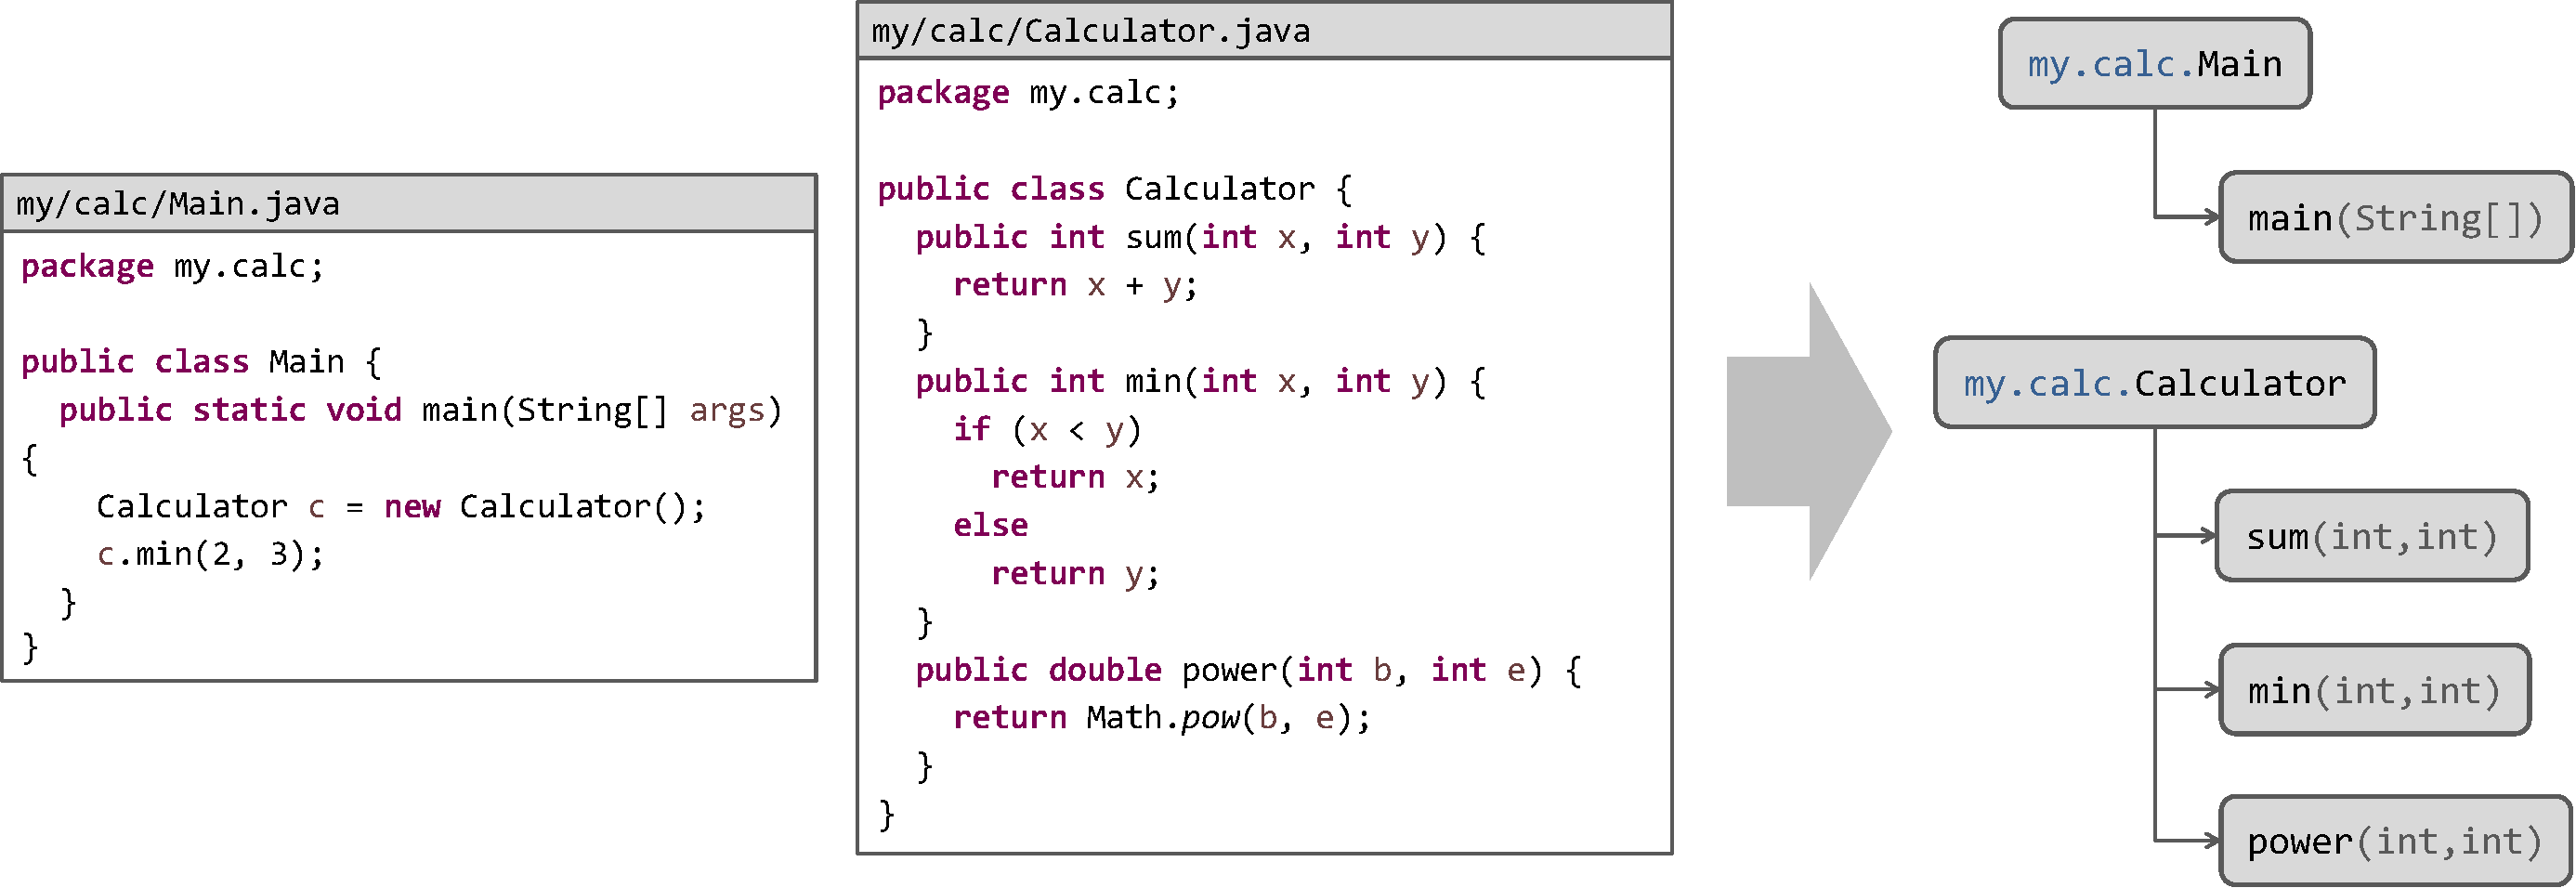
\includegraphics[width=1.0\textwidth]{img/javaToCst.pdf}
\caption{Transformation of the source code to CST}
\label{FigJavaToCst}
\end{figure*}

Along with each node of the CST, we store the following information:
\begin{description}
    \item[Identifier] \hfill \\
    An identifier of the code element in its declared scope. 
    The identifier is usually the name of the code element, but it may also contain additional information to avoid ambiguities.
    For example, the identifier of the class \codeinl{Calculator} from Figure~\ref{FigJavaToCst} is simply its name, but the identifier of the method \codeinl{add} is \codeinl{add(int,int)} because there could be an overloaded method with a different signature.
    
    \item[Namespace] \hfill \\
    An optional prefix that, along with the identifier, globally identifies the code element. 
    This information only applies to root nodes and corresponds to the package or folder that the element is contained. For example, the namespace of the class \codeinl{Calculator} from Figure~\ref{FigJavaToCst} is \codeinl{my.calc.}.
    
    \item[Node type] \hfill \\
    A string that identifies the node type in the target language (class, function, method, etc.).
    
    \item[Parameters list]  \hfill \\
    An optional list of the name of the parameters, in the case the node corresponds to a method or function.
    
    \item[Tokenized source code]  \hfill \\
    The source code of code element in the form of a list of tokens. 
    This information is necessary to compute the similarity between code elements, as explained in Section~\ref{SecCodeSim}.
    
\end{description}

In our approach, we generate the CST only for source files that have been added, removed, or modified between revisions. 
Such information can be efficiently obtained from version control systems, without the need to read the content of all files within the repository.
This way, we avoid a costly operation that might compromise the scalability of our approach, as large repositories contains thousands of source files, but only a small fraction of them change between subsequent revisions.

Besides the representation of the code elements, the CST also holds a simplified call graph and the type hierarchy of the nodes within the graph, that is, whether a certain node $n_1$ calls $n_2$, or $n_1$ is a subtype of $n_2$. The first information is necessary to find \emph{Extract} and \emph{Inline} relationships between code elements, while the second is used to find inheritance related relationships such as \emph{Pull Up} and \emph{Push Down}.


It is worth noting that the construction of the CST is a language-specific process, as we need to parse the source code, generate the AST for the target programming language, and extract the necessary information. However, from this point on, the approach is language-independent and relies only on the information encoded in the CST.
This way, one is able to extend our approach to work with different programming languages only by implementing the \emph{Source Code Analysis} module. To demonstrate that capability, we provide implementations for three programming languages: Java, C, and JavaScript.


\subsection{Phase 2: Relationship Analysis}


\begin{table*}[htbp]
\renewcommand{\arraystretch}{1.2}
\caption{Relationship types}
\label{TabRelationshipTypes}
\centering

\begin{tabular}{@{}lll@{}}
\toprule
Relationship type & Conditions \\
\midrule
& \multicolumn{2}{l}{$(n_1, n_2) \in N^- \times N^+$, such that:}\\
Same & & $\rdsig(n_1) = \rdsig(n_2) \land \rdparent(n_1)' = \rdparent(n_2) \land \rdtype(n_1) = \rdtype(n_2)$ \\
Convert type & & $\rdsig(n_1) = \rdsig(n_2) \land \rdparent(n_1)' = \rdparent(n_2) \land \rdtype(n_1) \neq \rdtype(n_2)$ \\
Pull Up & & $\rdsig(n_1) = \rdsig(n_2) \land \rdparent(n_1)' \neq \rdparent(n_2) \land \rdsub(\rdparent(n_1)', \rdparent(n_2))$ \\
Push Down & & $\rdsig(n_1) = \rdsig(n_2) \land \rdparent(n_1)' \neq \rdparent(n_2) \land \rdsub(\rdparent(n_2), \rdparent(n_1)')$ \\
Change signature & & $\rdname(n_1) = \rdname(n_2) \land \rdsig(n_1) \neq \rdsig(n_2) \land \rdparent(n_1)' = \rdparent(n_2) \land \rdsim(n_1, n_2) > \tau$ \\
Move & & $\rdname(n_1) = \rdname(n_2) \land \rdparent(n_1)' \neq \rdparent(n_2) \land \rdsim(n_1, n_2) > \tau$ \\
Rename & & $\rdname(n_1) \neq \rdname(n_2) \land \rdparent(n_1)' = \rdparent(n_2) \land \rdsim(n_1, n_2) > \tau$ \\
Move and Rename & & $\rdname(n_1) \neq \rdname(n_2) \land \rdparent(n_1)' \neq \rdparent(n_2) \land \rdsim(n_1, n_2) > \tau$ \\
\addlinespace
& \multicolumn{2}{l}{$(n_1, n_2) \in N_1^= \times N^+$, such that:}\\
Extract Supertype & & $\exists (n_3, n_4, \mathit{PullUp}) \in R_{1,2}\,|\,n_1 = \rdparent(n_3) \land n_2 = \rdparent(n_4)$ \\
Extract & & $\rduses(n_1', n_2) \land \rdparent(n_1)' = \rdparent(n_2) \land \rdsimx(n_2, n_1) > \tau$ \\
Extract and Move & & $\rduses(n_1', n_2) \land \rdparent(n_1)' \neq \rdparent(n_2) \land \rdsimx(n_2, n_1) > \tau$ \\
\addlinespace
& \multicolumn{2}{l}{$(n_1, n_2) \in N^- \times N_2^=$, such that:}\\
Inline & & $\rduses(n_1, n_2') \land \rdsimx(n_1, n_2) > \tau$ \\
\bottomrule
\end{tabular}

\vspace{1em}
\begin{tabular}{@{}lll@{}}
%\multicolumn{3}{c}{Legend}\\
\midrule
\begin{tabular}{@{}ll@{}}
$\rdname(n)$ & simple name of the code element $n$\\
$\rdsig(n)$ & identifier of the code element $n$\\
$\rdtype(n)$ & node type of the code element $n$\\
$\rdsub(n_1, n_2)$ & $n_1$ is subtype of $n_2$\\
$\rduses(n_1, n_2)$ & $n_1$ uses $n_2$\\
\end{tabular}
& &
\begin{tabular}{@{}ll@{}}
$\rdparent(n)$ & parent of a node $n$ (it may be a namespace or another CST node)\\
$n'$ & the code element that matches with $n$ in the other revision\\
$\rdsim(n_1, n_2)$ & similarity index between $n_1$ and $n_2$\\
$\rdsimx(n_1, n_2)$ & extract similarity index between $n_1$ and $n_2$\\
\end{tabular}
\\
\midrule
\end{tabular}

\end{table*}



This phase takes as input the CST's of revisions $v_1$ and $v_2$ and outputs the set of relationships $R_{1,2}$. Let $N_1$ and $N_2$ be the sets of code elements from the CST's of $v_1$ and $v_2$ respectively, each relationship $r \in R_{1,2}$ is a triple $(n_1, n_2, t)$, where $n_1 \in N_1$, $n_2 \in N_2$, and $t$ is a relationship type. The types of relationships are listed in the first column of Table~\ref{TabRelationshipTypes}, and can be subdivided into two groups:
\begin{enumerate}
\item \textbf{Matching relationships}, which include \textit{Same}, \textit{Convert type}, \textit{Pull Up}, \textit{Push Down}, \textit{Change signature}, \textit{Move}, \textit{Rename}, and \textit{Move and Rename}.
Those relationships indicates that the node $n_1$ corresponds to $n_2$ in the subsequent revision.

\item \textbf{Non-matching relationships}, which include \textit{Extract Supertype}, \textit{Extract}, \textit{Extract and Move}, and \textit{Inline}.
Those relationships don't indicate a matching, but rather that either node $n_1$ is decomposed to create $n_2$, or node $n_1$ is incorporated into $n_2$.
\end{enumerate}

Our approach employs an iterative procedure to find the relationships.
Let $N^-$ be the set of nodes from $N_1$ that were deleted and $N^+$ be the set of nodes from $N_2$ that were added.
Initially, we define $R_{1,2} \gets \emptyset$, $N^- \gets N_1$, and $N^+ \gets N_2$.
%That is, before finding any relationship, we consider that all code elements from $v_1$ were deleted and  all code elements from $v_2$ were created.
In each step, we look for pairs $(n_1, n_2)$ that match the criteria for a specific relationship type and add the corresponding relationships to $R_{1,2}$.
Additionally, we remove $n_1$ from $N^-$ and $n_2$ from $N^+$, in the case of a matching relationship.
By the end of the procedure, $R_{1,2}$ contains all relationships found, $N^-$ contains the removed nodes, and $N^+$ contains the added nodes.


\begin{itemize}
\item $N^-$ is the set of nodes from $N_1$ that were deleted.
\item $N^+$ is the set of nodes from $N_2$ that were added.
\item $N_1^=$ is the set nodes from $N_1$ that matches with another node from $N_2$, i.e., a node $n_1$ is in $N_1^=$ if exists a triple $(n_1, n_2, t) \in R_{1,2}$ such that $t$ is a matching relationship.
\item $N_2^=$ is the set nodes from $N_2$ that matches with another node from $N_1$ (analogously to $N_1^=$).
\end{itemize}



% Initialization
% Identity matching
% Top-level similarity matching
% Pull-up / Push down
% Low level similarity matching



\subsection{Code Similarity}
\label{SecCodeSim}

\begin{figure*}[htb]
\renewcommand{\arraystretch}{1.3}
\centering
\footnotesize
\begin{tabular}{@{}llll@{}}
\begin{tabular}{p{6.5cm}}
\multicolumn{1}{c}{\textbf{Source code of a class}} \\
\begin{lstlisting}
public class Calculator {

  public int sum(int x, int y) {
    return x + y;
  }

  public int min(int x, int y) {
    if (x < y) return x;
    else return y;
  }

  public double power(int b, int e) {
    return Math.pow(b, e);
  }
}
\end{lstlisting}\\

\end{tabular}
& {\Large $\Rightarrow$} &
\begin{tabular}{|l|r|r|r|}
\multicolumn{4}{c}{\textbf{Multiset of tokens for each method}} \\
\hline
Token $t$ & $m_{\mathtt{sum}}(t)$ & $m_{\mathtt{min}}(t)$ & $m_{\mathtt{power}}(t)$\\
\hline
\codeinl{return} & 1 & 2 & 1 \\
\codeinl{x}      & 1 & 2 & 0 \\
\codeinl{+}      & 1 & 0 & 0 \\
\codeinl{y}      & 1 & 2 & 0 \\
\codeinl{;}      & 1 & 2 & 1 \\
\codeinl{if}     & 0 & 1 & 0 \\
\codeinl{(}      & 0 & 1 & 1 \\
\codeinl{<}      & 0 & 1 & 0 \\
\codeinl{)}      & 0 & 1 & 1 \\
\codeinl{else}   & 0 & 1 & 0 \\
\codeinl{Math}   & 0 & 0 & 1 \\
\codeinl{.}      & 0 & 0 & 1 \\
\codeinl{pow}    & 0 & 0 & 1 \\
\codeinl{b}      & 0 & 0 & 1 \\
\codeinl{,}      & 0 & 0 & 1 \\
\codeinl{e}      & 0 & 0 & 1 \\
\hline
\end{tabular} &
\begin{tabular}{|r|}
\multicolumn{1}{c}{} \\
\hline
$n_t$\\
\hline
3 \\
2 \\
1 \\
2 \\
3 \\
1 \\
2 \\
1 \\
2 \\
1 \\
1 \\
1 \\
1 \\
1 \\
1 \\
1 \\
\hline
\end{tabular}
\end{tabular}
\caption{Transformation of the body of each method into a multiset of tokens}
\label{FigSourceCodeTransformation}
\end{figure*}

A key element of our approach to find relationships, as mentioned previously, is computing the similarity.
The first step to compute the similarity between code elements is to represent their source code as a multiset (or bag) of tokens.
A multiset is a generalization of the concept of a set, but it allows multiple instances of the same element.
The multiplicity of an element is the number of occurrences of that element within the multiset. Formally, a multiset can be defined in terms of a multiplicity function $m: U \to \mathbb{N}$, where $U$ is the set of all possible elements. In other words, $m(t)$ is the multiplicity of the element $t$ in the multiset. Note that the multiplicity of an element that is not in the multiset is zero.

For example, Figure~\ref{FigSourceCodeTransformation} depicts the transformation of the source code of three methods (\codeinl{sum}, \codeinl{min}, and \codeinl{power}), of the class \codeinl{Calculator}, into multisets of tokens. In this figure, the multiplicity function $m$ for each method is represented in a tabular form. For example, the multiplicity of the token \codeinl{y} in method \codeinl{min} is two (i.e., $m_{\mathtt{min}}(\mathtt{y}) = 2$), whilst the multiplicity of the token \codeinl{if} in method \codeinl{power} is zero (i.e., $m_{\mathtt{power}}(\mathtt{if}) = 0$).


Later, to compute the similarity between two code elements $e_1$ and $e_2$, we use a generalization of the Jaccard coefficient, known as weighted Jaccard coefficient~\cite{chierichetti2010finding}.
Let $U$ be the set of all possible tokens and $w(e, t)$ be a weight function of a token $t$ for the entity $e$.
We define the similarity between $e_1$ and $e_2$ by the following formula:


\begin{align}
\rdsim(e_1, e_2) = \frac{\sum_{t \in U} \min(w(e_1, t), w(e_2, t))}
                        {\sum_{t \in U} \max(w(e_1, t), w(e_2, t))}
\end{align}

%\subsubsubsection{Weight of a token for a code entity}

Our similarity function is based on a weighting function $w(e, t)$ that expresses the importance a token $t$ for a code entity $e$.
In fact, some tokens are more important than others to discriminate a code element.
For example, in Figure~\ref{FigSourceCodeTransformation}, all three methods contain the token \codeinl{return}. In contrast, only one method (\codeinl{power}) contains the token \codeinl{Math}. Therefore, the later is a better indicator of similarity between methods than the former.

In order to take this into account, we employ a variation of the TF-IDF weighting scheme~\cite{salton1986introduction}, which is a well-known technique from information retrieval.
TF-IDF, which is the short form of \emph{Term Frequency–Inverse Document Frequency}, reflects how important a term is to a document within a collection of documents.
In the context of code elements, we consider a token as a term, and the body of a method (or class) as a document.

Let $E$ be the set of all code elements and $n_t$ be the number of elements in $E$ that contains the token $t$,
we define the weight of $t$ for a code element $e$ as the function $w(e, t)$, which is defined by the following formula:
\begin{align}
w(e, t) = m_e(t) \times \mathit{idf}(t)
\end{align}

\noindent where $m_e(t)$ is the multiplicity of $t$ in $e$, and $\mathit{idf}(t)$ is the Inverse Document Frequency, which is defined as:
\begin{align}
\mathit{idf}(t) = \log (1 + \frac{|E|}{n_t})
\end{align}

Note that the value of $\mathit{idf}(t)$ decreases as $n_t$ increases, because the more frequent a token is among the collection of code elements, the less important it is to distinguish code elements.
For example, in Figure~\ref{FigSourceCodeTransformation}, the token \codeinl{y} occurs in two methods (\codeinl{sum} and \codeinl{min}). Thus, its $\mathit{idf}$ is:

\[
\mathit{idf}(\mathtt{y}) = 
\log (1 + \frac{|E|}{n_t}) = 
\log (1 + \frac{3}{2}) = 0.398
\]

On the other hand, the token \codeinl{else} occurs in one method ($\mathtt{min}$), and its $\mathit{idf}$ is:

\[
\mathit{idf}(\mathtt{else}) = 
\log (1 + \frac{|E|}{n_t}) = 
\log (1 + \frac{3}{1}) = 0.602
\]


\subsubsection{Extract and Inline Similarity}

While the similarity function presented previously is suitable to compute whether two code elements are are similar, in some situations we need to assess whether the source code of an element is contained within another one. This is the case of \emph{Extract}, and \emph{Inline} relationships. For example, if a method $e_2$ is extracted from $e_1$, the source code of $e_2$ should be contained within $e_1$ prior to the refactoring, although $e_1$ and $e_2$ may be significantly different from each other. Analogously, if a method $e_1$ is inlined into $e_2$, the source code of $e_1$ should be contained within $e_2$.
Thus, we defined a specialized version of the similarity function $\rdsimx$ defined by the following formula:
\begin{align}
\rdsimx(e_1, e_2) = \frac{\sum_{t \in U} \min(w(e_1, t), w(e_2, t))}
                        {\sum_{t \in U} w(e_1, t)}
\end{align}

The rationale behind this formula is that the similarity is at maximum when the multiset of tokens of $e_1$ is a subset of the multiset of tokens of $e_2$, i.e., all tokens from $e_1$ can be found in $e_2$. Note that, given this definition, $\rdsimx(e_1, e_2) \neq \rdsimx(e_2, e_1)$.


